\chapter{理論} \label{cha:theory}
\section{散乱断面積の計算の準備}
\subsection{ハドロン系の質量の仮定}
ハドロン中間状態の質量 $m_W$ は $\pi$ の質量$m_\pi$と陽子の質量 $m_p$の合計よりも大きくなければならない。

\begin{equation}
    m_W \geq m_\pi + m_p \approx 0.14 + 0.94 = 1.08 \ GeV
\end{equation}

よって、ハドロン系の質量は$m_W \geq 1.08$ GeVを仮定する。


\subsection{光子のエネルギーの仮定}
三元運動量を考える。\ref{fig:test2}
核子、光子の三元運動量をそれぞれ$p_N$, $p_\gamma$とすると、

\begin{equation}
    p_N = (0, m_N),\  p_\gamma = (E_\gamma, E_\gamma)
\end{equation}
とかけ、$m_W$との関係は

\begin{equation}
    m_W^2 = (p_N + p_\gamma)^2 = p_N^2 + 2p_N p_\gamma + p_\gamma^2
          = 2m_N E_\gamma + m_N^2 
\end{equation}
(1.3)式から$m_W$ = 1.08 GeV の時、$m_N$ = 0.94 GeVであるから

\begin{figure}[H]
	\centering
	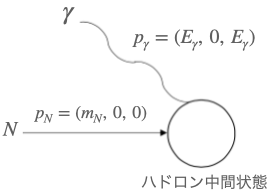
\includegraphics[width=10cm]{img/diagram_momentum.png}
	\caption{ハドロン中間状態と核子と光子の図}
	\label{fig:test2}
\end{figure}

\begin{equation}
    E_\gamma \approx 0.23 GeV
\end{equation}

よって、光生成反応を観測するために必要な光子のエネルギー$E_\gamma$は
$E_\gamma \geq 0.23 GeV$となる。

\subsection{宇宙線$\mu$の仮定}
宇宙線$\mu$ のエネルギー$E_\mu$ には$E_\gamma$ よりも遥かに大きいエネルギーを持つ必要がある。
そのため$E_\mu = 1.5$ GeV とおく。
また$E_\mu = 1.5$ GeV 以上となる$\mu$ の割合Rは$R \approx 0.56$ と頻度が高めである。\ref{fig:test3}

参考文献入れる。。。。。。。。。。。。。。。。。。。

\begin{figure}[H]
    \centering
    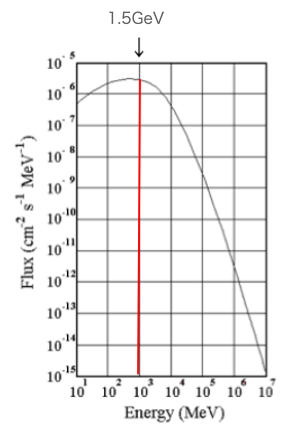
\includegraphics[width=10cm]{img/cosimic_ray_energy_distribution.png}
    \caption{宇宙線$\mu$のエネルギー分布}
    \label{fig:test3}
\end{figure}

$E_\mu$と散乱後の$\mu$のエネルギー$E'_\mu$ との比yとして、その値は
\begin{equation}
    y = \dfrac{E_\mu - E'_\mu}{E_\mu} \approx 0.2
\end{equation}

\section{生成断面積の計算枠組み}
$\mu$とNの散乱断面積$\sigma_{\mu N}$は$\mu$から$\gamma$を出す確率$\Phi$と、
$\gamma$とNとの散乱断面積$\sigma_{tot}(\gamma^* N)$の積で表すことができる。

\begin{equation}
    \sigma_{\mu N} =\int dy  \sigma_{tot}(\gamma^* N) \Phi(y)
\end{equation}

また、$\Phi(y)$は以下のように表す。
\begin{equation}
    \Phi(y) = \dfrac{\alpha}{\pi y} \int \dfrac{dQ^2}{Q^2} [(1-y)(1 - \dfrac{Q^2_{min}}{Q^2}) + \dfrac{y^2}{2}]
\end{equation}

$Q^2$を運動量移行の2乗の負数とした。


\section{\texorpdfstring{$\Phi$}{LG}の考察}
$\Phi$の積分前の関数は下のようになる。\ref{fig:test4}
\begin{figure}[H]
    \centering
    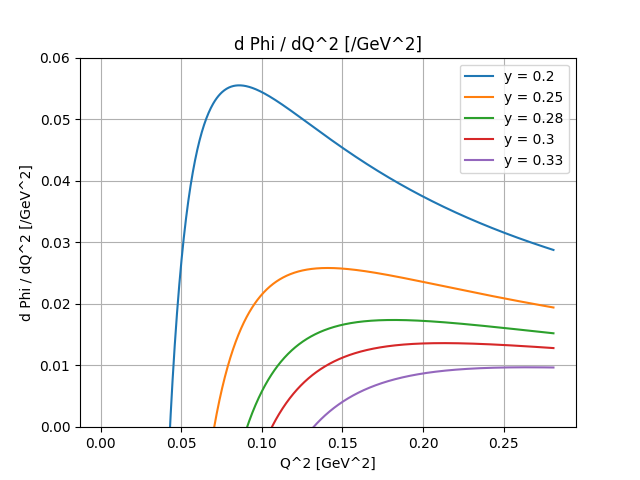
\includegraphics[width=10cm]{img/flux_fixed_y.png}
    \caption{$\dfrac{d\Phi ^2}{dydQ^2}$ のyを定数としたグラフ}
    \label{fig:test4}
\end{figure}

このグラフから$\Phi$はyが小さいところで大きくなる。つまり、$E_\mu$ が $E_\gamma$より遥かに大きくなるところで$\sigma_{\mu N}$が大きくなる。
また、$Q^2$が小さくなるところで大きくなっている。$Q^2$は0でない最小値を持つ。


\section{断面積の計算に用いる近似}
$\E_gamma = [300, 500]$MeVと仮定する。
下図を用いて$\gamma$とNの反応断面積$\sigma{tot}\gamma^* N$を
$\sigma{tot}\gamma^* N = 0.3$ mbと近似する。\ref*{fig:test5}
\begin{figure}[H]
    \centering
    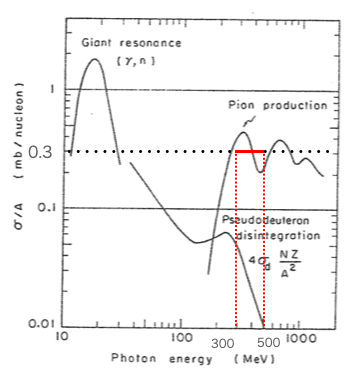
\includegraphics[width=10cm]{img/sigma_tot.png}
    \caption{核子1個あたりの全光核反応断面積と光子のエネルギーの関係}
    \label{fig:test5}
\end{figure}

$E_mu = 1.5$GeV,$E_\gamma = [0.3, 0.5]$GeVの仮定からyの範囲は$y = [0.20, 0.33]$となる。


\section{断面積に用いた式}
$m_W$の関係式$m_W = \sqrt{m_p^2 + 2m_pE_\mu y - Q^2}$は$m_w = 1.08$GeVとした時、下のようになる。\ref{fig:test6}

\begin{figure}[H]
    \centering
    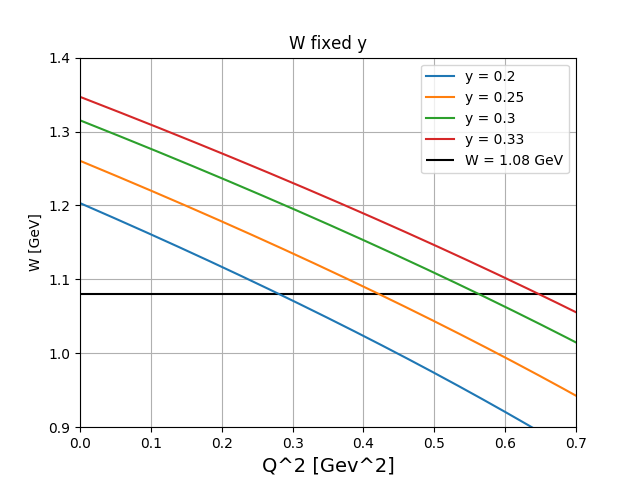
\includegraphics[width=10cm]{img/W2_fixed_y.png}
    \caption{$m_W = \sqrt{m_p^2 + 2m_pE_\mu y - Q^2}$のyを固定した関係式}
    \label{fig:test6}
\end{figure}

$m_w = 1.08$GeVの直線とyの値ごとの直線が交わる$Q^2$の値が$Q^2$の最大値となる。